% Sinh boi runners/make_paper1_figures.py; caption doi chieu bang
% runners/audit_figures.py. File rieng cho tung hinh de \input DUNG CHO
% trong than bai -- float cua LaTeX chi troi VE SAU, khai bao het o cuoi
% tai lieu thi ca 9 hinh don xuong cuoi va tran vao danh muc tai lieu.

\begin{figure*}[t]
  \centering
  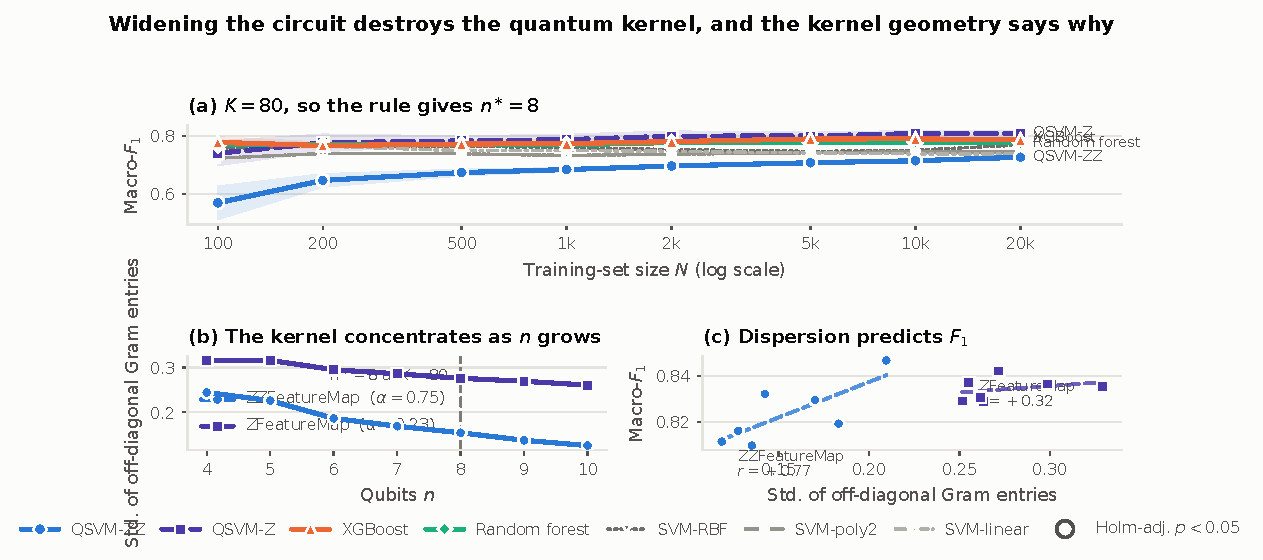
\includegraphics[width=\textwidth]{figs_revision/fig12_width_concentration.pdf}
  \caption{%
    \textbf{Widening the circuit destroys the quantum kernel, and the kernel
    geometry says why.} (a) The sample-complexity sweep re-run at $K=80$, where
    the rule returns $n^{\ast}=8$: all $48$ paired comparisons are
    classical-favourable. (b) Off-diagonal Gram dispersion against width, fitted
    as $n^{-\alpha}$ at $K=80$; the \ZZ{} map concentrates $3.3$ times as fast
    as the \Zmap{} map here ($\alpha=0.75$ against $0.23$), against the factor
    of $2.02$ at $K=20$ that phase-term counting predicts (Sec.~\ref{sec:res-width}).
    (c) Across widths the dispersion correlates with macro-$F_1$ at $r=+0.77$
    for \ZZ{} (95\% CI $[+0.04,+0.96]$) and $r=+0.32$ for \Zmap{}
    ($[-0.57,+0.87]$); the contrast between the two is not resolved at seven
    widths ($z=0.97$, $p=0.33$).}
  \label{fig:width}
\end{figure*}
